\section{Planning}
\SectionPage

\begin{frame}
  \frametitle{Features}
  \begin{itemize}
    \item Easy to extend (with modules)
      \pause
      \begin{itemize}
        \item Low bar to create a module
          \pause
        \item Easy to reason about how modules work together
          \pause
      \end{itemize}
    \item Proof-of-concept modules should extend the application to include
      these features:
      \pause
      \begin{itemize}
        \item Can open, edit, delete files
          \pause
        \item Has LSP support
          \pause
        \item Can compile and execute a program
      \end{itemize}
  \end{itemize}
\end{frame}

\begin{frame}
  \frametitle{Goals}
  % TODO: Should probably make these points more concrete
  \begin{itemize}
    \item Should be better than the current IDE
      \pause
      \begin{itemize}
        \item Easy installation
      \end{itemize}
      \pause
    \item Easy for the next \sout{sucker} developer to change core functionality
      \pause
      \begin{itemize}
        \item Good CI-CD
        \pause
        \item Good documentation
        \pause
      \end{itemize}
    \item Have a good module developer experience
      \begin{itemize}
          \pause
        \item Language Agnostic Module Architecture
          \pause
        \item Good debugging tools
      \end{itemize}
  \end{itemize}
\end{frame}

\begin{frame}
  \frametitle{What Is A Module?}
  \begin{itemize}
    \item Third Party Code to be executed/interpreted
      \pause
      \begin{itemize}
        \item Tailor made Scripting Language
          \pause
          \begin{itemize}
            \item Vim Script (Vim)
              \pause
          \end{itemize}
        \item An already existing programming language
          \pause
          \begin{itemize}
            \item Lua (Neovim)
          \end{itemize}
      \end{itemize}
  \end{itemize}
\end{frame}

\begin{frame}
  \frametitle{Granularity}
  \begin{itemize}
    \item How \textit{big} is a module?
      \pause
      \begin{itemize}
        \item Could create an IDE module which does everything
          \pause
          \begin{itemize}
            \item Not very granular
          \end{itemize}
          \pause
        \item Could create a module for each function
          \begin{itemize}
              \pause
            \item Very granular
          \end{itemize}
      \end{itemize}
  \end{itemize}
\end{frame}

\hidelogo
\begin{frame}
  \frametitle{Module Family}
  \begin{itemize}
    \item Grouping of related modules that work together.
      \pause
    \item Example
      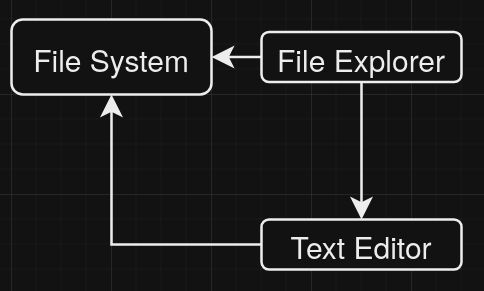
\includegraphics[width=0.9\textwidth]{./pics/ide-family.png}
  \end{itemize}
\end{frame}

\showlogo
\section{Modeling a Module}
\SectionPage

\begin{frame}
  \frametitle{How To model A Module?}
  \begin{itemize}
    \item A module needs to:
      \pause
      \begin{itemize}
        \item Initialize some state
          \pause
        \item Update the state based on events
          \pause
        \item Change the view based on the state
      \end{itemize}
      \pause
    \item Module architecture is inspired by Elm and MVC
      \pause
    \item A module should be \textit{pure}
  \end{itemize}
\end{frame}

\begin{frame}
  \frametitle{Module V.1}
  \begin{itemize}
    \item First plan
      \pause
      \begin{enumerate}
        \item Create an IDE
          \pause
        \item Extend the IDE, to allow for a module architecture
          \pause
        \item Modules call the application using some DSL
          \pause
      \end{enumerate}
    \item Pros
      \pause
      \begin{itemize}
        \item \textit{Easy} to implement
          \pause
        \item Get a good understanding of what features might be needed
          \pause
      \end{itemize}
    \item Cons
      \pause
      \begin{itemize}
        \item Not really modular
          \pause
        \item Will be subpar compared to existing software
      \end{itemize}
  \end{itemize}
\end{frame}

\begin{frame}
  \frametitle{Module V.1 - Final}
  \begin{itemize}
    \item Second plan
      \pause
      \begin{enumerate}
          % TODO: Add footnote
        \item Everything* is a module
      \end{enumerate}
      \pause
      \begin{itemize}
        \item A module exposes three functions, that are invoked by the core
          \pause
          \begin{itemize}
            \item Init - Returns a set of fields, which are added to the core state
              \pause
            \item Update - Returns a set of fields which are updated
              \pause
            \item View - Returns a set which represents HTML, which is rendered by
              the Core
          \end{itemize}
          \pause
        \item Pros
          \pause
          \begin{itemize}
            \item Easy to keep modules pure
              \pause
            \item Optimization is possible due to the pureness of modules
              \pause
            \item Easy to reason about module cooperation
          \end{itemize}
          \pause
        \item Cons
          \pause
          \begin{itemize}
            \item State is append-only
              \pause
            \item State can only grow
              \pause
            \item Not really modular
          \end{itemize}
      \end{itemize}
  \end{itemize}
\end{frame}

\begin{frame}
  \frametitle{Example Types for State}
  \begin{minted}{haskell}
data Value
  = VInt Int
  | VStr String
  | VBool Bool
  | VFloat Float
  | VLst [Value]
  | VObj [(String, Value)]

newtype State = [(String, Value)]
\end{minted}

\end{frame}

\begin{frame}
  \frametitle{Example Types for Msg and HTML}
  \begin{minted}{haskell}
data Msg = Msg
  { msg :: String
  , val :: Value
  }

data HTML
  = Div [Attributes] [HTML]
  | Btn [Attributes] [ Html]
  | Text String
  -- ...

data Attributes
  = OnClick Msg
  | Id String
  -- ...
\end{minted}

\end{frame}

\hidelogo
\begin{frame}
  \frametitle{Example}
  \begin{minted}{haskell}
-- Manifest :: Map
init :: Map
init :: [("counter", ValInt 0)]

update :: Msg -> Map -> Map
update (PluginMsg "counter") model =
  case lookup "counter" model of
    Just (ValInt i) -> insert "counter" (ValInt (i + 1)) model
    Nothing -> insert "counter" (ValInt 0) model

view :: Map -> Html
view model = Div [] [Text "Hello, World!"
  , Btn [OnClick (PluginMsg "counter")] []
  , Text (putStrLn (lookupOrDefault "counter" model))
\end{minted}



\end{frame}

\showlogo
\begin{frame}
  \frametitle{Module V.1 - Final.Final}
  \begin{itemize}
    \item Third, and hopefully the final plan
      \pause
      \begin{enumerate}
          % TODO: Add footnote
        \item Everything* is a module
          \pause
        \item Modules can \textit{invoke} modules
          \pause
      \end{enumerate}
      \begin{itemize}
        \item Init - Returns a set of modifications
      \end{itemize}
      \pause
    \item Pros
      \pause
      \begin{itemize}
        \item Modular
          \pause
        \item Modules can \textit{invoke} other modules
      \end{itemize}
      \pause
    \item Cons
      \begin{itemize}
          \pause
        \item Complex to implement
      \end{itemize}
  \end{itemize}
\end{frame}

\begin{frame}
  \frametitle{Example}
  \begin{minted}{haskell}
data Module = Module
  { name :: String
  , init :: Core -> CoreModification
  }
\end{minted}

\end{frame}


\begin{frame}
  \frametitle{Example Event}
  \begin{minted}{haskell}
newType EventHandler = Event -> Core -> CoreModification

data Event = Event
  { moduleName :: String
  , eventName :: String
  , arguments :: Maybe Value
  }

\end{minted}

\end{frame}


\begin{frame}
  \frametitle{Example Counter}
  \begin{minted}{haskell}
module :: Module
module = Module { name = "Counter", init }

counterEvent :: Event
counterEvent = Event
  { moduleName = "CounterModule"
  , eventName = "Counter"
  , arguments = Just $ VInt 1
  }

init :: Core -> CoreModification
init core = emptyCoreModification
  { uiModification =
    [ AddUI $ Btn [Id "CounterBtn", OnClick counterEvent] [Text "Click"]
    ]
  , stateModification = [AddField "Counter" (ValInt 0)]
  , eventHandler = [("Counter", evtHdl)]
  }
\end{minted}

\end{frame}


\begin{frame}
  \frametitle{Example Counter Handler}
  \begin{minted}{haskell}
evtHdl :: Event -> Core -> CoreModification
evtHdl evt c = case (eventName evt, arguments evt) of
  ("Counter", (Just i)) -> emptyCoreModification
    { stateModification = [UpdateField "Counter" (\x -> x + i)]
    }
  _ -> emptyCoreModification
\end{minted}

\end{frame}

% TODO: Talk more about the complexity, like with tree-changes and such
